\subsection*{Genome assembly of three medaka strains}
  Three medaka inbred strains were recently sequenced with PacBio single-molecule real-time (SMRT) sequencing and were assembled by the author's laboratory (Ichikawa \textit{et al}., unpublished; see Methods for an overview of the assembly procedure). Two strains (Hd-rR and HNI) were established from northern and southern Japanese populations, respectively and the other one (HSOK) was established from eastern Korean population. The two Japanese populations are estimated to have separated 18 million years ago (MYA), whereas the ancestor of the two Japanese populations and that of the eastern Korean population are estimated to have separated 25 MYA \cite{Setiamarga2009}.

  % NOTE: move this subsection to the introduction?


\subsection*{Genomic abundance of centromeric repeats}
  This study started with a candidate centromeric satellite sequence of medaka which was identified in a previous computational study \cite{Melters2013}. In that study, Melters \textit{et al.} estimated that the candidate centromeric satellite comprise 0.32\% of the medaka genome. However this estimation can underestimate the true genomic abundance due to its identification strategy. In order to better infer the genomic abundance of the centromeric satellite, PacBio raw reads were searched for the centromeric satellite sequence.

  Genomic fraction of the centromeric repeat was estimated by searching PacBio subreads for the representative monomer sequence with RepeatMasker \cite{}. The genomic fraction in Hd-rR and HNI genomes were estimated to be $\sim$1\%, while that in the HSOK genome was $\sim$2\% (Table \ref{centromeric_repeat_genomic_abundance}). This difference is consistent with the previous observations that centromeric repeat array size in a chromosome can vary up to 20-fold among individuals within a species \cite{Miga2014}. Assuming the genome size to be 800 Mb, the centromeric satellite comprise 8--16 Mb of the genome, which implies each chromosome has around 500 kb of centromeric satellite on average. This is concordant with the observations that the centromere of many higher eukaryotes studied to date are characterized by hundreds to thousands of kilobases of satellite sequences \cite{Plohl2014}. Although quantifying the centromeric satellite in erroneous PacBio reads can lead to slight underestimation, the estimation should be more reliable than the clustering-based estimation using short Sanger reads in the previous study \cite{Melters2013}.

  % TODO: add citation of RepeatMasker


\subsection*{Centromeric repeat distribution}
  The distribution of centromeric repeats in the three medaka strain genomes were revealed by searching their genomes using RepeatMasker (Table \ref{centromeric_repeat_distribution}). For those chromosomes that have $>$1 kb centromeric repeat, positions of the centromeres in chromosomes were classified into metacentric, submetacentric, subtelocentric and acrocentric, employing the nomenclature by Levan \textit{et al}. \cite{levan1964} (Table \ref{centromeric_repeat_distribution}). Although this nomenclature originally based on karyotype observation rather than DNA sequence level and the positions induced from the two levels can slightly differ, the sequence-based classification conducted here is  nevertheless informative for interpreting subsequent analyses. The number of chromosomes classified to each type was in line with previous karyotype studies \cite{}.

  % TODO: add citation to the karyotype study or the book.

  \begin{table*}[htp]
    \centering
    \caption{Centromeric repeat distribution}
    \begin{tabular}{r|rc|rc|rc}
  \hline
  & \multicolumn{2}{c|}{Hd-rR} & \multicolumn{2}{c|}{HNI} & \multicolumn{2}{c}{HSOK} \\ \hline
  chromosome & total repeat (bp) & position & total repeat (bp) & position & total repeat (bp) & position \\ \hline
  1  & 48,805  & SM  & 0      & -  & 0       & -  \\
  2  & 54,844  & M   & 3,831  & M  & 64,213  & M  \\
  3  & 52,681  & ST  & 0      & -  & 0       & -  \\
  4  & 10,513  & A   & 0      & -  & 305,521 & M  \\
  5  & 0       & -   & 10,605 & A  & 0       & -  \\
  6  & 8,226   & A   & 1,635  & A  & 7,020   & A  \\
  7  & 0       & -   & 12,911 & A  & 25,917  & A  \\
  8  & 59,863  & SM  & 0      & -  & 324,346 & SM \\
  9  & 40,159  & SM  & 0      & -  & 0       & -  \\
  10 & 0       & -   & 14,685 & ST & 0       & -  \\
  11 & 4,755   & A   & 4,513  & A  & 66,412  & A  \\
  12 & 232,280 & SM  & 25,683 & SM & 40,516  & SM \\
  13 & 35,778  & A   & 0      & -  & 0       & -  \\
  14 & 33,284  & A   & 0      & -  & 0       & -  \\
  15 & 0       & -   & 0      & -  & 63,112  & A  \\
  16 & 12,804  & A   & 0      & -  & 0       & -  \\
  17 & 1,588   & A   & 0      & -  & 0       & -  \\
  18 & 23,853  & SM  & 0      & -  & 9,236   & SM \\
  19 & 131,040 & SM  & 4,830  & SM & 4,757   & SM \\
  20 & 96,309  & ST  & 0      & -  & 17,574  & ST \\
  21 & 87,124  & M/A & 2,131  & A  & 0       & -  \\
  22 & 61,066  & A   & 0      & -  & 4,942   & A  \\
  23 & 6,580   & M   & 0      & -  & 25,847  & SM \\
  24 & 0       & -   & 0      & -  & 0       & -  \\
  \hline
  anchored total & 1,001,552 &  & 80,824 &  & 959,413 \\
  unanchored total & 3,279,256 & (5.89\%) & 2,254,882 & (3.16\%) & 11,273,168 & (17.5\%) \\
  total & 4,280,808 &  & 2,335,706 &  & 12,232,581 \\
  \hline
  positions summary & \multicolumn{2}{c|}{2M+6SM+2ST+8A (6U)} & \multicolumn{2}{c|}{1M+2SM+1ST+5A (15U)} & \multicolumn{2}{c}{2M+5SM+1ST+5A (11U)} &
  \hline
\end{tabular}

    \label{centromeric_repeat_distribution}
    \caption*{{\small
      RepeatMasker hits against the medaka centromeric satellite were collected over each chromosome. The centromeric positions were determined by repeat distribution on chromosomes employing the nomenclature by Levan \textit{et al} \cite{Levan1964}. Note that Hd-rR chromosome 21 possessed centromeric repeat arrays of nearly the same length (41.6 kb and 45.5 kb) at the positions corresponding to metacentric and acrocentric, thus described as 'M/A'. M, metacentric; SM, submetacentric; ST, subtelocentric; A, acrocentric; U, unknown (due to the lack of centromeric repeats).
    }}
  \end{table*}

  Centromeric positions of the same chromosome were mostly conserved among the strains, confirmed by observing the corresponding pair of genetic markers flanked the repeat arrays, with only two exceptions in chromosomes 4 and 6 (Fig. \ref{genome_browser}). For chromosome 4, Hd-rR had an acrocentric repeat array, whereas HSOK had a metacentric array. For chromosome 6, all the three strains had acrocentric repeat arrays but those of Hd-rR and HSOK and that of HNI located on the opposite end of the chromosome. As the karyotype study has revealed that the three strains possess slightly different sets of centromeric positions \cite{}, the difference of chromosomes 4 and 6 may be derived from \textit{bona fide} karyotype difference. Of note, Hd-rR chromosome 21 possessed metacentric and acrocentric arrays of nearly the same length (41.6 kb and 45.5 kb, respectively; Fig. \ref{genome_browser}), thus this chromosome may dicentric where one of the arrays forms the functional centromere whereas the other is silenced.

  % TODO: describe that assemblies truncated at centromeric repeat arrays and no chromosomal arrays were completely spanned.
  % TODO: describe that substantial amount of centromeric repeats were contained in unanchored contigs.
  % NOTE: provide centromeric positions from the karyotype study as a supplementary table?


\subsection*{Centromeric sequence mapping by FISH}
  To confirm that the candidate centromeric satellite sequence truly localizes to the centromeres, FISH experiment was conducted. Probe sequences were designed by the author and FISH experiments were carried out by a collaborator (see Methods).

  The candidate satellite was first used as a hybridization probe and signals were observed only from 5$\sim$7 pairs of chromosomes. Additional probes were designed to complement hybridization to other chromosomes. For each chromosome, satellite monomers were collected from satellite arrays and the collected monomers were aligned back to the original array with BLASTN \cite{}. Then a monomer with the highest score was chosen as the representative monomer of the chromosome, where the score was defined as:

  % TODO: add citation of BLAST

  \[
    score = \sum_{\mbox{hits}} \mbox{alignment identity} \cdot \frac{\mbox{alignment length}}{\mbox{query length}}.
  \]

  Representative monomers obtained from each chromosome were then aligned to the Hd-rR genome with BLASTN and three monomers that exhibited high identity to different subsets of chromosomes were chosen as additional probe sequences (Fig. \ref{}). The additional probes successfully hybridized to some chromosomes that the first probe failed to hybridize, although two additional probes hybridized to less number of chromosomes than expected from the \textit{in silico} alignment results. When all the probes combined, signals were observed at the centromeres of $\sim$13 pairs of chromosomes (Fig. \ref{fish_all}). This result confirmed that the candidate centromeric satellite truly derives from the centromeres. Moreover, the number of the chromosomes having each centromeric positions were largely consistent with the sequence-based results in the previous section.

  \begin{figure*}[htp]
    \centering
    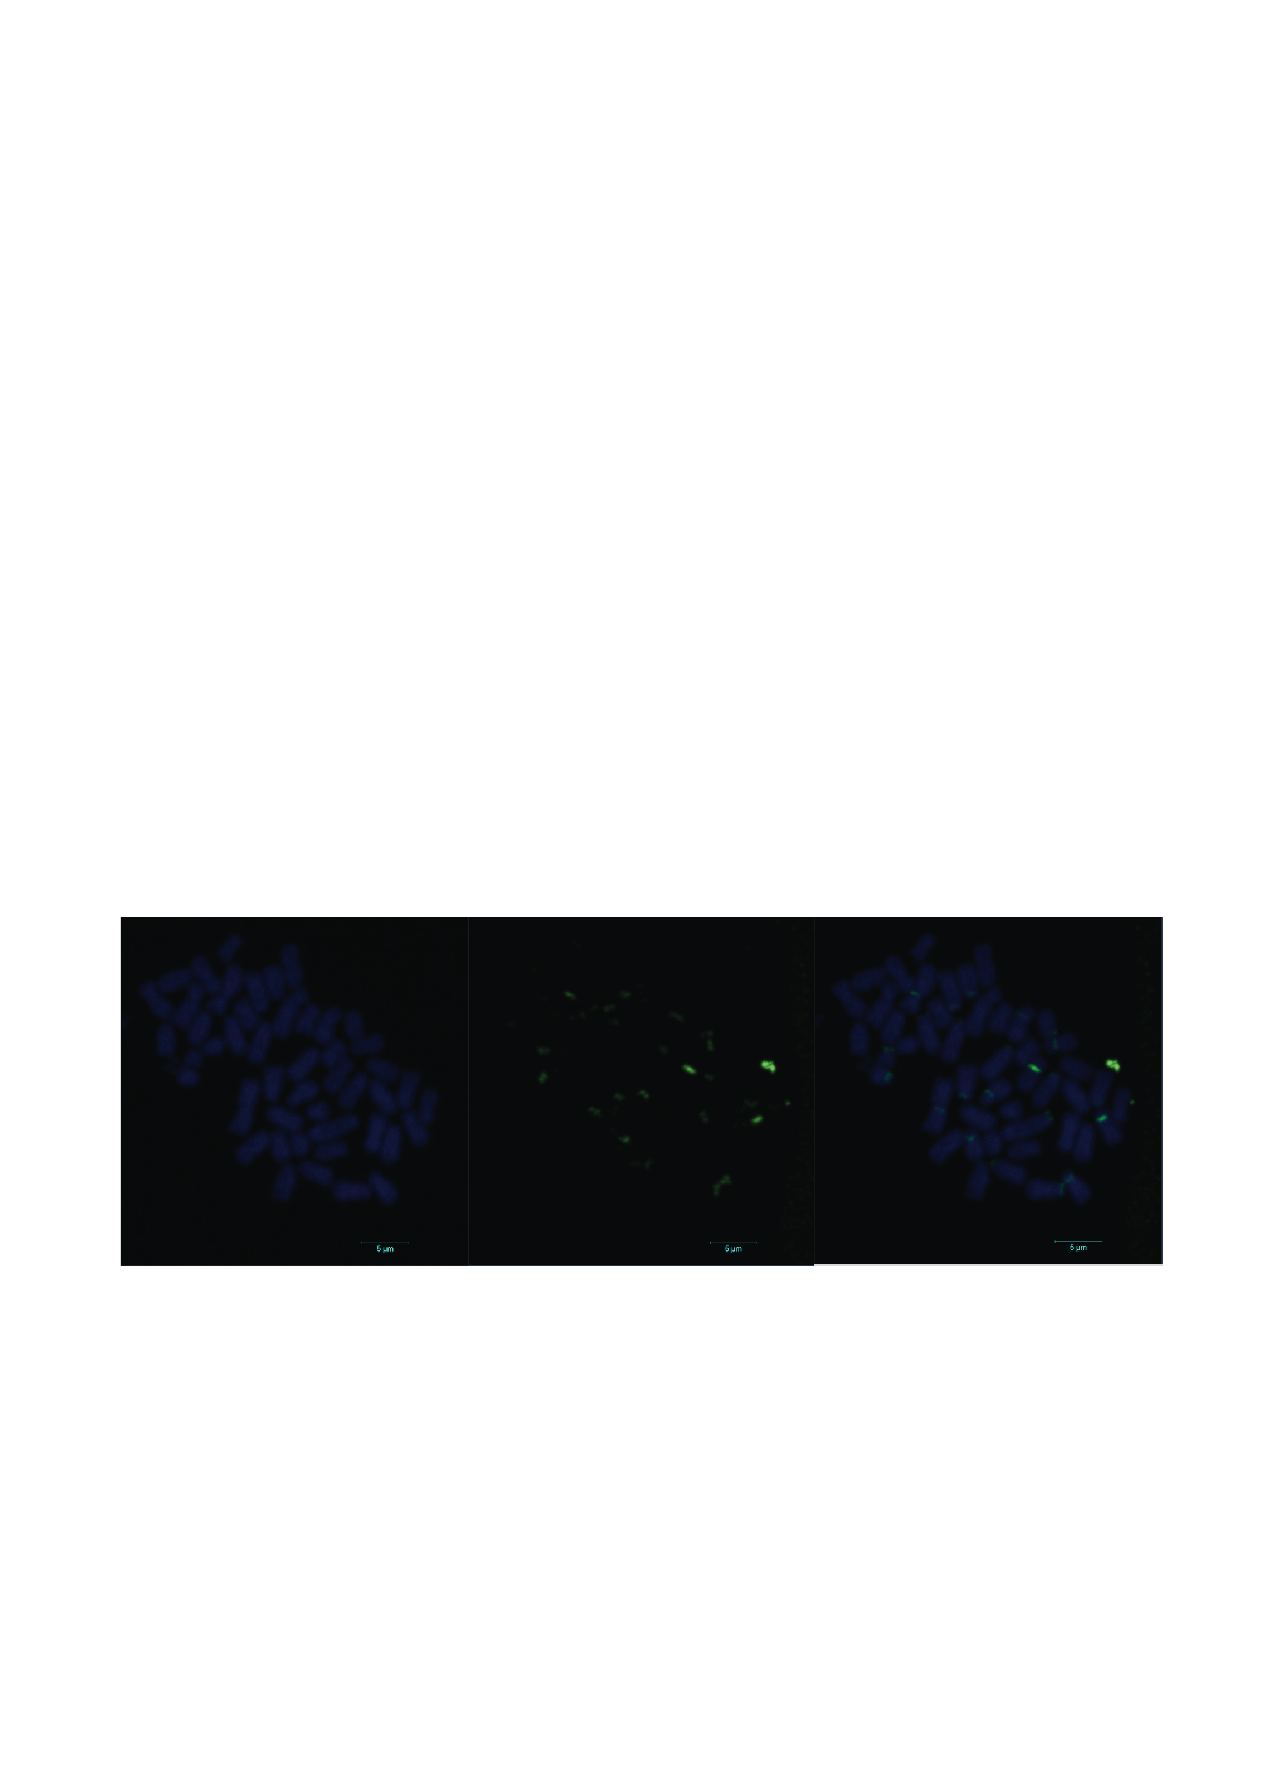
\includegraphics[width=\linewidth]{fish_all_probes.pdf}
    \caption{
      The candidate centromeric satellite sequence and three derivative sequences localized to the centromeres of $\sim$13 pairs of chromosomes. (left) DNA is stained with DAPI. (center) probes are stained green. (right) two images are combined.
    }
    \label{fish_all}
  \end{figure*}


\subsection*{Validation of centromeric sequence assembly}
  Repetitive nature of centromeric sequences inevitably accompanies the possibility of misassembly. In order to validate the centromeric sequence assembly, PacBio raw subreads were mapped to the assembled genomes and read coverage over centromeric regions was visually inspected on a genomic browser.

  PacBio subread were mapped to the medaka genomes by BLASR \cite{} with a stringent mapping parameters (see Methods). The assembly validity was then visually inspected on the genomic browser by confirming that enough number of subreads covered the centromeric repeat arrays without breaks. Most part of the centromeric sequences were covered by enough number of subreads, although a small number of exceptions were observed in chromosomes 9, 13 and 20 in the Hd-rR genome, which contained one or two breaking points that were not spanned by subreads (Supplementary Fig. \ref{centromere_landscape}). Although PacBio read-based assembly validation cannot completely exclude the possibility of misassembly, indeed long-range ordering over the centromeric repeat arrays can be inaccurate, nevertheless relatively narrow range of assembly can be ascertained and that is adequately informative for observing sequence composition of a specific chromosome or inter-chromosomal sequence similarity.


\subsection*{Inter-chromosomal centromeric sequence conservation}
  Previous studies have revealed that centromeric sequences exhibit inter-chromosomal conservation that are considered to be derived from evolutionary process of chromosome formation \cite{}. In order to reveal the presence of inter-chromosomal relationship of centromeric repeats in medaka genomes, chromosomal-representative satellite monomers were collected and clustered.

  Specifically, centromeric repeat arrays in each chromosome were decomposed into satellite monomers by RepeatMasker and the monomers were clustered by DNACLUST \cite{} with $>$85\% sequence similarity threshold. For those clusters that have $\geq$10 members, the monomer with the longest sequence in the cluster was chosen as the representative monomer of the cluster. All-vs-all pairwise alignment of the representative monomers from each chromosome along with the representative monomer identified by Melters \textit{et al}. was performed and the distance between the monomers were calculated. Based on this distance, hierarchical clustering of the chromosome-representative monomers were performed (Fig. \ref{monomer_clustering}). The chromosome-representative monomers were clustered into four groups, revealing the presence of super-chromosomal subfamilies (Table \ref{super_chromosomal_subfamily}). Many (15 out of 24) chromosomes (chr. 2, 3, 5, 6, 7, 10, 11, 12, 14, 15, 16, 18, 20, 22 and 23) were assigned exclusively to one of the four subfamilies. Five chromosomes (chr. 1, 4, 8, 13 and 19) were clustered into two or three subfamilies but significantly more monomers were classified to one subfamily over others, thus assigned to the dominant subfamily. Chromosomes 9 and 21 were classified into two subfamilies with no significant preference. Chromosome 17 and 24 were not able to be classified due to the lack or insufficient amount of centromeric repeats in either of the three assembled genomes. Overall, 22 out of 24 chromosomes were assigned to one or two subfamilies. Intriguingly, each subfamily exhibited distinct preference of centromeric positions in chromosomes; namely subfamily 1 for acrocentric, subfamily 2 and 3 for submetacentric and subtelocentric and subfamily 4 for metacentric, respectively (Table \ref{super_chromosomal_subfamily}).

  % TODO: Add description on sequence conservation of acrocentric chromosomes in the human genome to support the result. (Willard 1991)

  In those chromosomes that had sufficient amount of centromeric repeats in multiple strains, most (7 out of 9) chromosomes were classified into the same subfamilies among strains. One of the exceptions was chromosome 19, where representative monomers from Hd-rR and HSOK were classified into SF2 while that of HNI into SF3, although the repeats from each strain were confirmed to locate in close position of the chromosome as they were flanked by a corresponding pair of genetic markers (Supplementary Fig. \ref{genome_browser}). This discordant classification may be due to assembly of different subregion of the corresponding repeat array among strains or may have been caused by misassembly in one or more strains. The other exception was chromosome 21, where the representative monomers from the acrocentric array of Hd-rR were classified into SF1, those from the metacentric array of Hd-rR and from the acrocentric array of HNI into SF3. The two acrocentric arrays from Hd-rR and HNI were located at close but distinct positions in the chromosome (Supplementary Fig. \ref{genome_browser}), thus it may as well contain different repeat sequence profiles and be classified into different subfamilies.

  % TODO: Describe the consistency with Melters's result that centromeric sequence are conserved in species within 50MYA after separation.

  \begin{figure*}
    \centering
    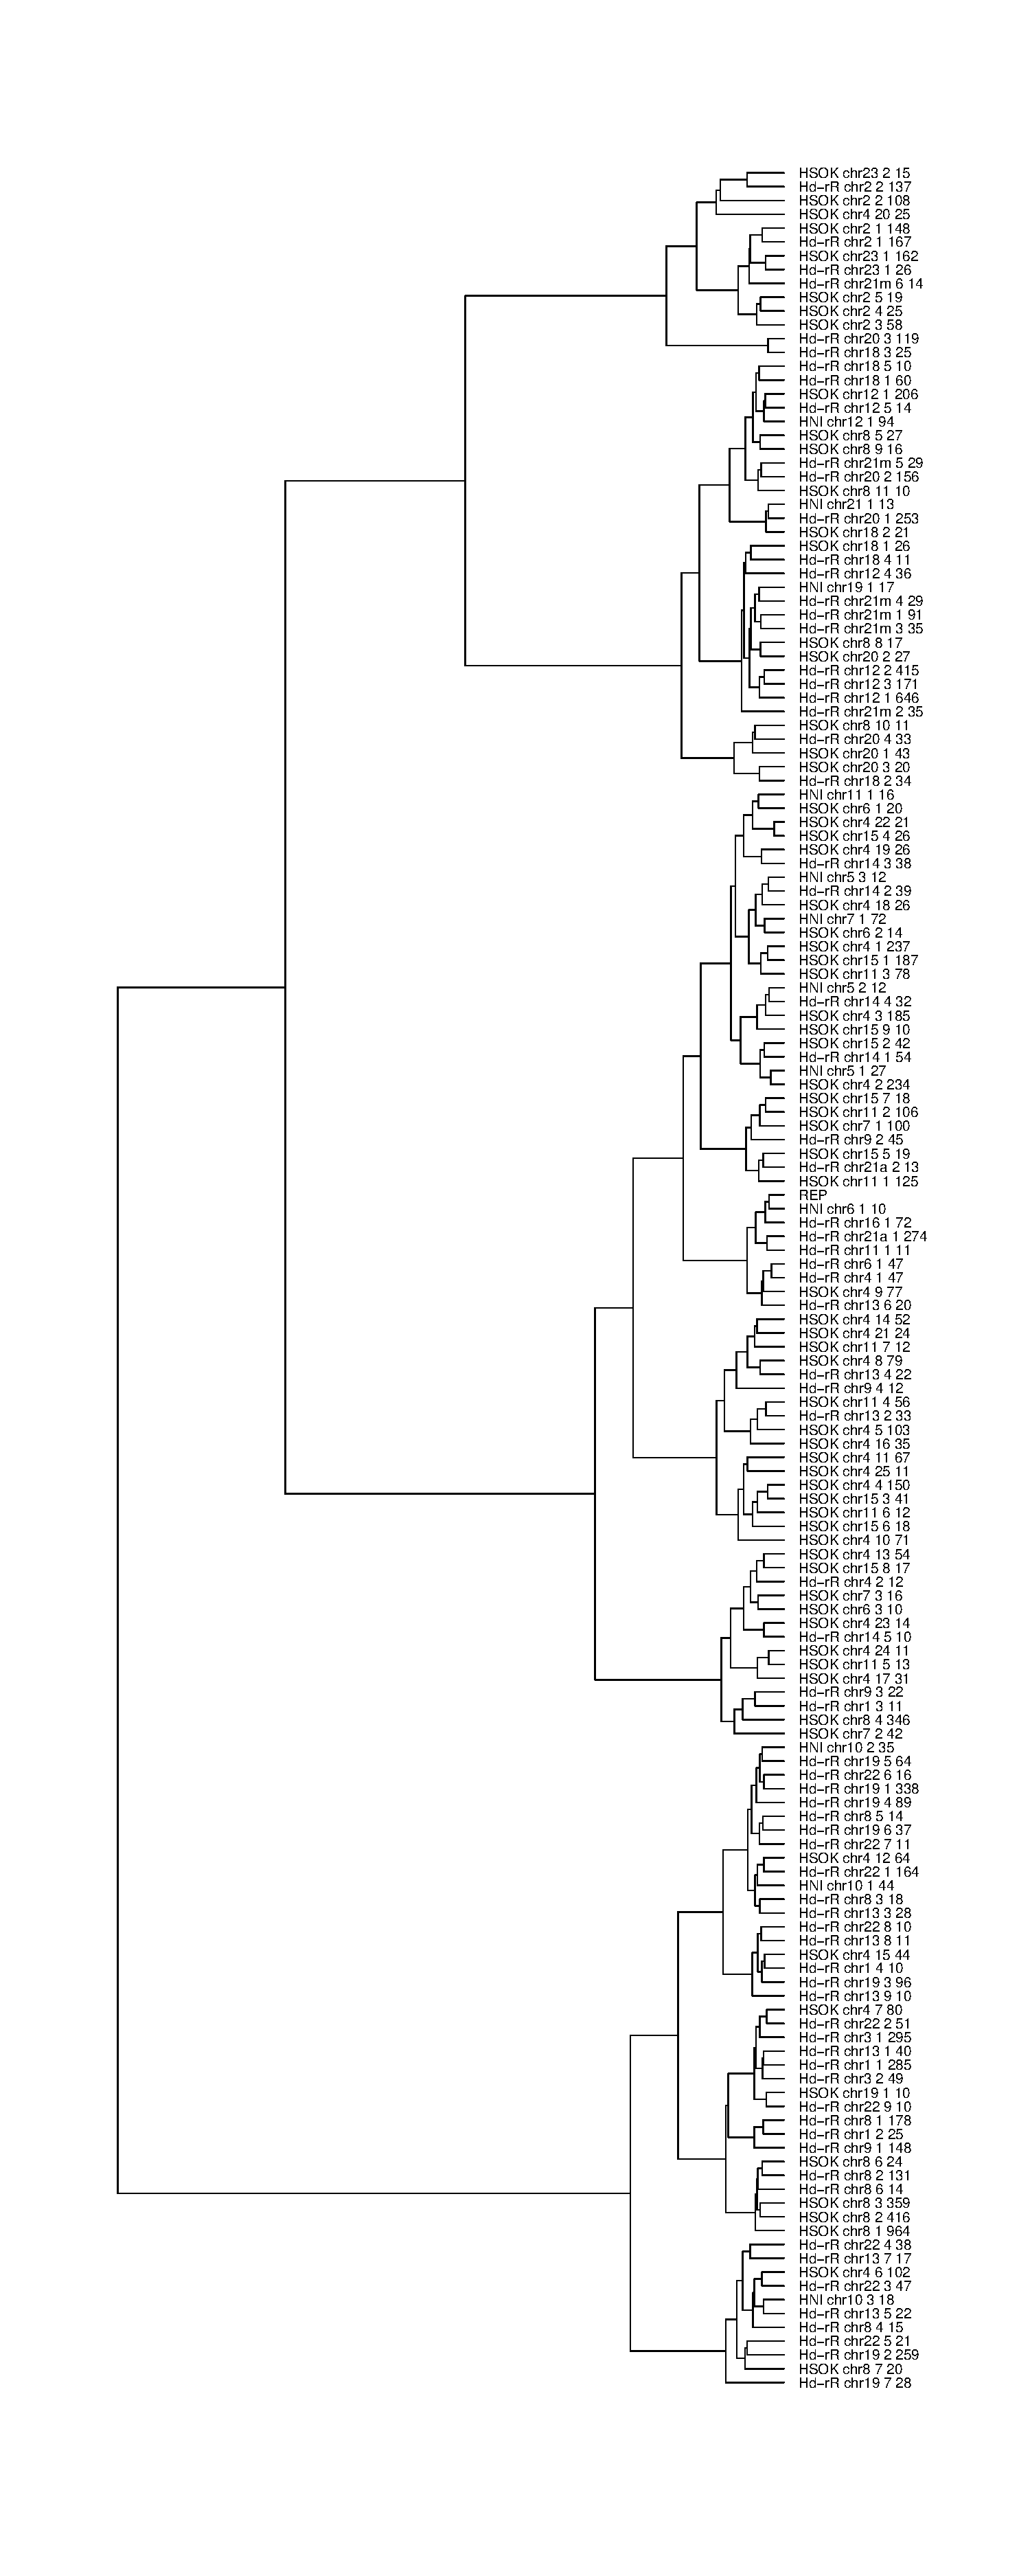
\includegraphics[width=0.5\linewidth]{representative_monomers_clustering.pdf}
    \caption{
      Hierarchical clustering of chromosome-representative monomers. Monomers are labeled as species, chromosome, cluster index, number of the cluster constituents.
    }
    \label{monomer_clustering}
  \end{figure*}
  % TODO: replace the figure with a nice one!

  \begin{table*}
    \centering
    \caption{Super-chromosomal subfamilies of centromeric repeats}
    \begin{tabular}{p{0.6cm}p{3.4cm}p{1.5cm}p{2cm}p{4.5cm}p{3.7cm}}
  \hline
  SF & Hd-rR & HNI & HSOK & combined & positions \\ \hline
  1 & 4,6,9,11,14,16,21a (1,13) & 5,6,7,11    & 4,6,7,11,15 (8) & 4,5,6,7,9,11,14,15,16,21a (1,8,13) & 1M+1SM+14A (2SM+1A) \\
  2 & 1,3,8,9,13,19,22          & 10          & 8,19 (4)        & 1,3,8,9,10,13,19,22 (4)            & 6SM+2ST+2A (1M) \\
  3 & 12,18,20,21m (8)          & 12,21 (19)  & 12,18,20 (8)    & 12,18,20,21m (8,19)                & 1M+8SM+2ST+1A (2SM) \\
  4 & 2,23 (21m)                &             & 2,23 (4)        & 2,23 (4,21m)                       & 3M+1SM (2M) \\
  \hline
\end{tabular}

    \label{super_chromosomal_subfamily}
    \caption*{{\small
      Chromosomes were classified into four subfamilies (SF). Chromosomes in brackets are the ones that have significantly more amount of repeats classified into another subfamily. Hd-rR chromosome 21 possessed two distantly-positioned arrays, thus is notated as 21m (metacentric) and 21a (acrocentric; see Table \ref{centromeric_repeat_distribution} for detail). Summarizing the chromosomes from the three strains, 22 out of the 24 chromosomes were assigned to one or two subfamilies. Notation of the centromeric positions are the same as Table \ref{centromeric_repeat_distribution}.
    }}
  \end{table*}
